\documentclass{article}

% ready for submission
% \usepackage{neurips_2023}

% to compile a preprint version, e.g., for submission to arXiv, add add the
% [preprint] option:
\usepackage[preprint]{neurips_2023}

% to compile a camera-ready version, add the [final] option, e.g.:
%     \usepackage[final]{neurips_2023}

\usepackage[utf8]{inputenc} % allow utf-8 input
\usepackage[T1]{fontenc}    % use 8-bit T1 fonts
\usepackage{hyperref}       % hyperlinks
\usepackage{url}            % simple URL typesetting
\usepackage{booktabs}       % professional-quality tables
\usepackage{amsfonts}       % blackboard math symbols
\usepackage{nicefrac}       % compact symbols for 1/2, etc.
\usepackage{microtype}      % microtypography
\usepackage{xcolor}         % colors
\usepackage{graphicx}       % figures

\graphicspath{ {figures/} }

\title{QwinSR: An All-MLP Shifted Window Model for Image Super Resolution}

\author{
  Mark Bauer \\
  Siebel Department of Computer Science\\
  University of Illinois Urbana-Champaign\\
  \texttt{markb6@illinois.edu} \\
  \And
  Quinn Ouyang\thanks{"QwinSR" is a play on Swin using Quinn's name. This was Mark's idea.} \\
  School of Music \\
  University of Illinois Urbana-Champaign \\
  \texttt{qouyang3@illinois.edu} \\
}

\begin{document}

\maketitle

\begin{abstract}
    Since its inception, the Swin Transformer backbone architecture has consistently showcased remarkable performance across a range of well-established computer vision benchmarks. To enhance computational efficiency, the Swin Mixer architecture has adopted a similar structure. However, it distinguishes itself by substituting transformers with Mixer Layers, thus giving rise to Swin Mixer Layers (SMLs). In line with this design, we introduce QwinSR, an application of this all-MLP architecture tailored for the task of single image super-resolution. This adaptation simplifies the original transformer-based image restoration model, SwinIR. QwinSR leverages SMLs to extract essential features and subsequently aggregates them within a compact convolutional neural network, facilitating image reconstruction. We anticipate that this approach will yield competitive accuracy-to-computation ratios, particularly when compared to SwinIR and other leading models in the field.
\end{abstract}

\section{Introduction}

Despite advances in modern photography and image transmission technology, resolution loss is often an unavoidable or necessary compromise. This produces a need and desire for techniques to construct higher fidelity images from lower resolution sources, which we call super resolution (SR) imaging. However, SR is a more niche category than other computer vision tasks (such as classification and semantic segmentation []), making this field ripe for new research. Given the simple objective and need for research on SR, we propose a simplified all-MLP model based on the shifted window design from Swin Transformer: QwinIR.

\subsection{Related Work}

\subsubsection{Single Image Super-Resolution}

“Super-resolution” generally refers to the process of enhancing the visual detail and fidelity of an image by predicting pixels to increase its resolution []. In other literature, SR is roughly interchangeable with the more general terms “upsampling” and “reconstruction.” Note that the latter implies that an exact / true higher resolution image exists for a lower resolution one, which typically comes from artificial downsampling (classic image SR) []. “Single image”  differentiates from the other common variant of this task, multiple image SR, which assumes the advantage of having more than one source image. Effective techniques exploit the related images for more pixel information to construct from, which can apply in the real-world (e.g. a burst shot, video frames, etc.) []. However, we focus on single image SR as it is a more fundamental and challenging task.

Traditional algorithmic approaches for SR directly interpolate pixels from a lower resolution source, typically assuming a downsampling process to generalize the reconstruction. Popular basic algorithms include bicubic and nearest-neighbor interpolation which are fast and eschew the long training times associated with learning-based models, but the absence of trained priors obviously limits their ability to hallucinate new pixels [].

\subsubsection{Learning-based Approaches}

On the other hand, learning-based models spanning a variety of architectures have far surpassed the generalized interpolations that traditional approaches limit themselves to [], as we briefly illustrated in Figure~\ref{fig:example}. Models based on convolutional neural networks (e.g. SRCNN, SRResNet), general adversarial networks (e.g. ESRGAN, SRGAN, Real-ESRGAN), and transformers (e.g. SwinIR) have all effectively competed for state-of-the-art performance [].

\begin{figure}\label{fig:example}
    \centering
    \begin{tabular}{c c c c}
        
\includegraphics[width=80pt]{bicubic.png} & 
\includegraphics[width=80pt]{srresnet.png} & 
\includegraphics[width=80pt]{srgan.png} & 
\includegraphics[width=80pt]{original.png} \\
        \small Bicubic Interpolation              & \small SRResNet                            & \small SRGAN                            & \small Original
    \end{tabular}
    \caption{Visual comparisons of traditional and learning-based classic image SR approaches to a $\times 4$-upscaled original high resolution image.}
\end{figure}

For SR related tasks, CNNs are effective at global feature extraction but have lately been usurped by transformers, which tend to be more robust and lightweight. As a consequence, pure CNN models often require added complexity just to match the performance of transformer models [https://arxiv.org/pdf/2105.01601.pdf]. It is quite common to utilize hybrid CNN-transformer models, in which CNNs are used for global feature extraction while transformers focus on local feature extraction []. E.g. …

GANs tend to be tedious to fine tune and also have many trainable parameters, making the training process very long []. Similarly, diffusion models like StableSR have gigantic datasets and are quite complex []. The focus of this research project is on simplicity, and as such we do not consider these models.

\subsubsection{All-MLP}

“All-MLP” describes a model as primarily relying on only multi-layer perceptrons (MLPs), often in contrast to neural networks or transformers. These models tend to have significantly fewer parameters and simpler architectures to offer an ideal tradeoff between accuracy and training time / running time [mlp mixer, swin t]. Proposed by Tolstikhin et al., the MLP-Mixer is one of the first all-MLP demonstrations for computer vision. Despite its apparent computational limitations, MLP-Mixer has boasted results comparable to those from state-of-the-art implementations for image classification. Inspired by this work, we chose to follow the same all-MLP design philosophy and apply it on SR as a more high level benchmark.

\subsubsection{Shifted Window}

\paragraph{Swin Transformer:} First popularized by Liu et al., the shifted window approach is the computational representation in a groundbreaking computer vision model: the Swin Transformer. Critically, it limits “self-attention computation to non-overlapping local windows while also allowing for cross-window connection,” eliminating global self-attention and thus reducing from quadratic to linear computational complexity relative to image size [swin t]. Variants of the Swin Transformer have achieved state-of-the-art results in a variety of common tasks, including image classification and semantic segmentation [3].

\paragraph{Swin-Mixer:} The modularity of the shifted window technique in the Swin Transformer enables replacing its attention layers with MLPs, yielding the Swin-Mixer. Specifically, it replaces each of its multi-head attention layers with the all-MLP layers presented by Tolstikhin et al., converting the Swin Transformer blocks into Swin Mixer blocks. Swin-Mixer surpasses the already classification results of MLP-Mixer and other all-MLP models [swin t, mlp mix], but little research exists on how it performs elsewhere, e.g. in SR.

\paragraph{SwinIR:} A pioneering model for attention-based SR, SwinIR uses basic convolutional layers for shallow feature extraction and Swin Transformer blocks for deep feature extraction. These extracted features are then passed through a basic upsampling convolution that involves a convolutional layer and a pixel shuffle. SwinIR impressively surpasses other top-performing models based on CNNs, GANs, etc. in classical SR [swin ir].

\section{Model Architecture}

\begin{figure}\label{fig:architecture}
    \centering
    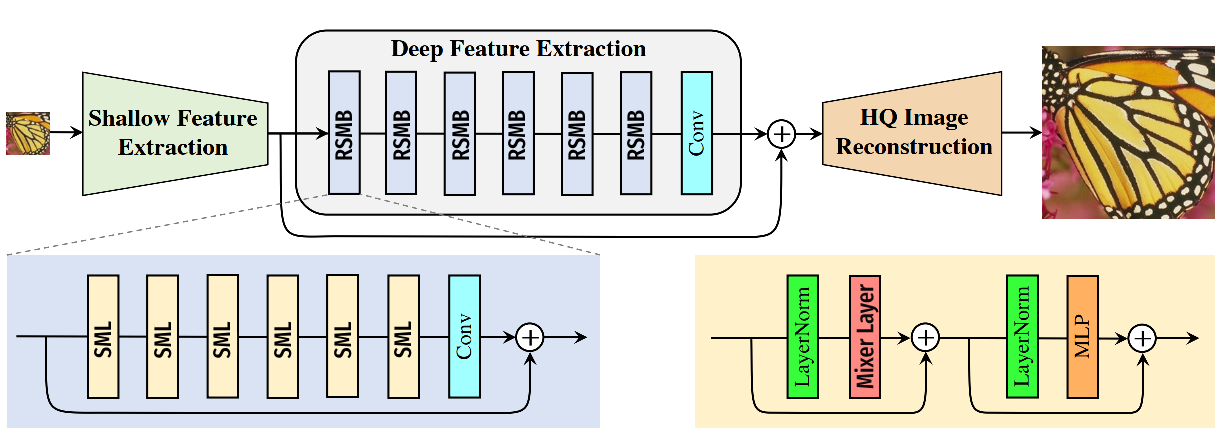
\includegraphics[width=\textwidth]{qwinir-architecture.png}
    \caption{The architecture of QwinIR. Figure based off of that of SwinIR.}
\end{figure}

The architecture of QwinIR is novel, in that it combines the model architectures of SwinIR and Swin-Mixer. Similar to SwinIR, our model involves a 3 step architecture: shallow feature extraction, deep feature extraction, and image reconstruction. We illustrate this in Figure~\ref{fig:architecture}.

\subsection{Shallow Feature Extraction}

QwinIR uses the exact same method for shallow feature extraction as SwinIR. That is, given a low quality input image, we use a $3 \times 3$ convolutional layer to perform shallow feature extraction. This step is taken because convolutional layers are quite good at local feature extraction, making them useful in the early stages of image processing. The authors of the SwinIR paper note that the use of this layer not only leads to more stable optimization and better results, but it also provides a simple way of mapping input images to higher dimensional feature spaces [3].

\subsection{Deep Feature Extraction}

\begin{figure}\label{fig:transformer}
    \centering
    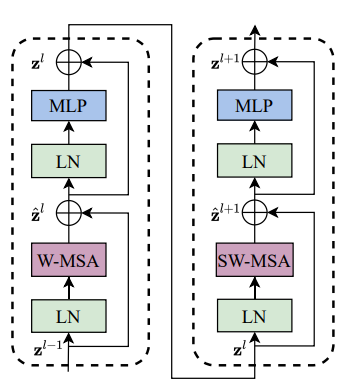
\includegraphics[width=100pt]{swin-transformer-block.png}
    \caption{Two original successive Swin Transformer blocks with attention heads included (W-MSA and SW-MSA). Swin Mixer blocks replace each of these with a Mixer Layer.}
\end{figure}

Next, we perform deep feature extraction by passing the extracted shallow features through a series of residual Swin mixer blocks (RSMBs) and a $3 \times 3$ convolutional layer (these blocks are called "residual" because they each contain a skip connection, where the results of each block are aggregated with the input features passed to the block). Each RSMB contains a series of Swin mixer layers (SMLs) followed by a $3 \times 3$ convolutional layer, and each Swin mixer layer is simply a Swin Transformer layer that has had its multi stage attention head replaced with a mixer layer, as we depict in Figure~\ref{fig:transformer} [4].

\paragraph{Mixer Layer:} Each mixer layer is composed of 2 MLPs, with two fully connected layers and GELU nonlinearities. Mixer layers contain one channel-mixing MLP and one token-mixing MLP. The channel-mixing MLPs come first, which allow communication between different input channels and operate on each input token independently. The results of the channel-mixing MLPs are passed to the token-mixing MLPs, which allow communication between different tokens and operate on each channel independently [14]. By utilizing this mixing architecture, features are able to be extracted without the explicit need for attention. Hence, it makes logical sense for deep feature extraction to be accurate even when attention heads in the Swin Transformer blocks are replaced with mixer layers. However, due to the removal of attention heads, these blocks are technically no longer transformers, and hence we do not refer to them as such.

\begin{figure}\label{fig:mixer}
    \centering
    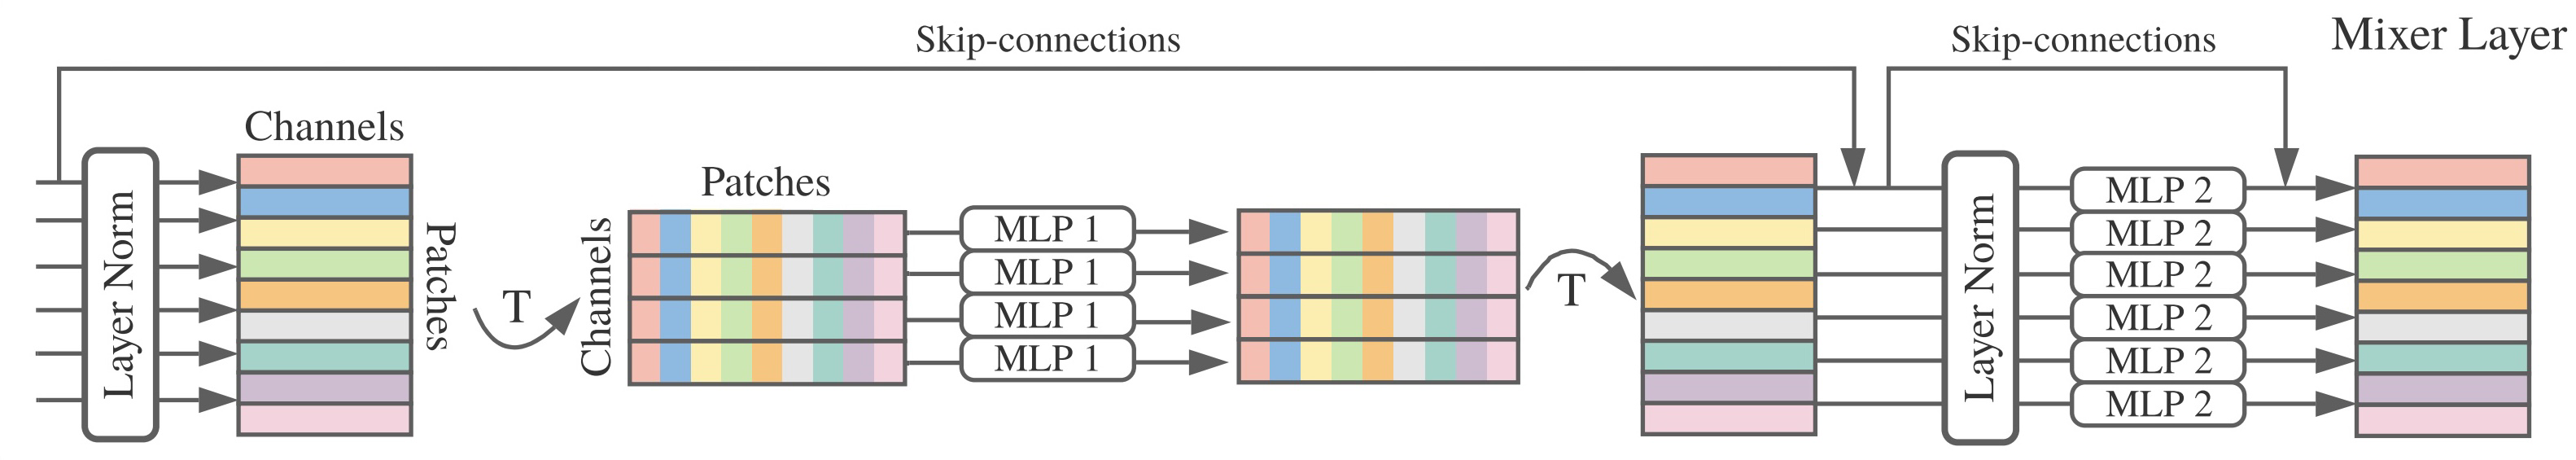
\includegraphics[width=\textwidth]{mixer-layer.png}
    \caption{Mixer layer from MLP-Mixer, consisting of token-mixing MLP, channel-mixing MLP, skip-connections, dropout, and layer normalization}
\end{figure}

\subsection{Reconstruction}

Using a skip connection, the originally extracted shallow features and the newly extracted deep features are aggregated and passed into an image reconstruction module. By using a skip connection, we can ensure that high frequency features are not lost during the reconstruction process [3]. For image reconstruction, we implement a sub-pixel convolutional neural network (ESPCN), the same technique utilized by SwinIR [7]. The ESPCN consists of two convolution layers for feature extraction, and a sub-pixel convolution layer that aggregates the low resolution features. From here, the ESPCN then constructs the high resolution image in a single step.

\begin{figure}\label{fig:escpn}
    \centering
    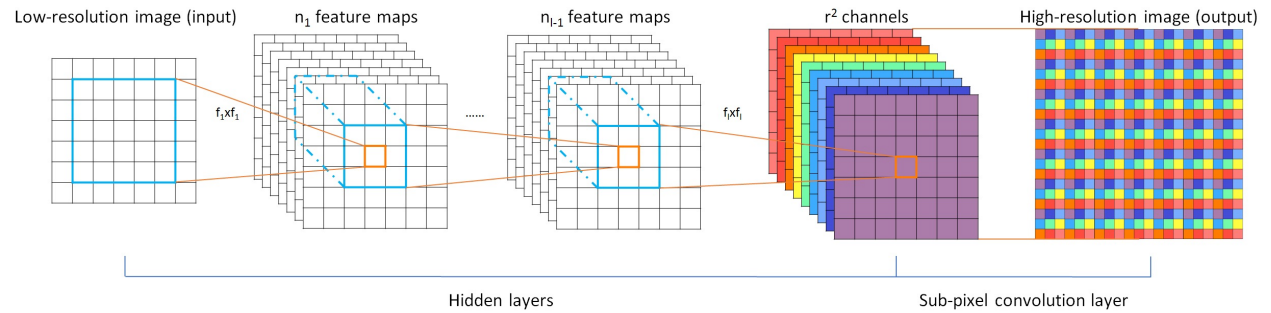
\includegraphics[width=\textwidth]{espcn.png}
    \caption{The network architecture for ESPCN}
\end{figure}

\section{Experiments}

Unfortunately, we were unable to conduct a formal experimental procedure due to resource and time constraints However, barring those factors, our experimental phase would proceed as follows: for our experimental procedure, we intend to test the ability of our model to perform image upscaling. Given that our model is derived from the SwinIR architecture, it is logical for our experiments to replicate those performed in the SwinIR paper. It should be noted that in the original SwinIR paper, the experimental procedure consists of image super resolution, image denoising, and JPEG compression artifact reduction. Since our architecture focuses only on super resolution, we ignore the other 2 experimental components.

\paragraph{Ablation Study:} The first stage of our experimental procedure will be an ablation study. This study involves altering and removing certain components from our model to understand the contributions of those components to our results. In this stage, our model will be trained on the DIV2K [11] dataset and will be tested on the Manga109 [12] dataset. The first portion of this stage will observe the effects of changing the channel number, number of Swin-MLP blocks, and number of SMLs per block on model performance. To perform this step, we will test a variety of combinations for values of these hyperparameters and observe the relative correlations between the values of each hyperparameter and peak signal to noise ratio (PSNR) for the upscaled images. The second portion of this stage will observe the effects of changing patch size and the number of training images. To perform this step, we will test a variety of combinations for values of these hyperparameters and observe how each value affects PSNR and time for convergence. The third portion of this stage will observe the effects of the residual connection and convolutional layer in each SMB. Like in the SwinIR paper, we will test 4 residual connection variants in each block: no residual connection (i.e. no convolution operation), a $1 \times 1$ convolution layer, a $3 \times 3$ convolution layer, and three $3 \times 3$ convolution layers. For each of these hyperparameter values, the corresponding PSNRs will be assessed and compared.

\paragraph{Results} In the second stage of our experimental procedure, we will select the optimal combination of hyperparameters as determined in the previous stage, and we will use them to test our model on the Set5 [8], Set14 [9], BSD100 [10], Urban100 [13], and Manga109 [12] datasets. The benchmarks we record in this stage will be PSNR (peak signal to noise ratio, lower indicates less grainy output images), SSIM (structural similarity index measure, which compares how similar an upscaled image is to the original high quality image a model seeks to reproduce), the number of model parameters, and the number of multiply-accumulate operations. These measurements will be compared to the benchmarks recorded in the SwinIR paper (this is convenient, because the SwinIR paper contains benchmarks for numerous SOTA architectures, not just for the SwinIR architecture). By performing this comparison, we will gain conclusive evidence as to how our model performs relative to state of the art models–in particular, if our model has a viable accuracy/cost ratio.

\section{Conclusion}

In this paper we propose QwinIR, an image restoration model that combines the architectures of SwinIR and Swin-Mixer. Like SwinIR, this model consists of three phases: shallow feature extraction, deep feature extraction, and image reconstruction. Unlike SwinIR, our model uses residual Swin-Mixer blocks for deep feature extraction, where each block consists of Swin-Mixer layers, a convolution layer, and a residual connection. While we were unable to conduct a formal experimental phase due to resource and time constraints, we believe that this model has potential to perform at a similar level to state of the art image upscaling models. For future work, we would like to conduct a formal testing phase on a more substantial cluster of GPUS, as GCP and our personal computers proved to be insufficient for training our model. Furthermore, we would like to experiment with the placement of skip connections within our network to potentially remove the need for an initial convolutional layer for shallow feature extraction, similar to the SwinSeg architecture described by Zhang et al. [6].

\begin{ack}
    We would like to acknowledge Paris Smaragdis, Krishna Subramani (please be gentle to us), Evan Matthews, Nicolas Prate, and Quinn’s sister’s cat, Sesame.
    
    We have no funding.
\end{ack}
\section*{References}

 [1] Alexander, J.A.\ \& Mozer, M.C.\ (1995) Template-based algorithms for
connectionist rule extraction. In G.\ Tesauro, D.S.\ Touretzky and T.K.\ Leen
(eds.), {\it Advances in Neural Information Processing Systems 7},
pp.\ 609--616. Cambridge, MA: MIT Press.


    [2] Bower, J.M.\ \& Beeman, D.\ (1995) {\it The Book of GENESIS: Exploring
        Realistic Neural Models with the GEneral NEural SImulation System.}  New York:
TELOS/Springer--Verlag.


[3] Hasselmo, M.E., Schnell, E.\ \& Barkai, E.\ (1995) Dynamics of learning and
recall at excitatory recurrent synapses and cholinergic modulation in rat
hippocampal region CA3. {\it Journal of Neuroscience} {\bf 15}(7):5249-5262.

[1] https://arxiv.org/pdf/1501.00092.pdf (SRCNN)

[2] https://arxiv.org/pdf/1609.04802.pdf (SRGAN)

[3] https://arxiv.org/pdf/2108.10257.pdf (SwinIR)

[4] https://arxiv.org/pdf/2103.14030.pdf (Swin Transformer)

[5] https://ieeexplore.ieee.org/stamp/stamp.jsp?tp=\&arnumber=1203207 (Overview)

[6] https://www.sciencedirect.com/science/article/pii/S0029801823012696?via=ihub (SwinSeg)

[7] https://arxiv.org/pdf/1609.05158.pdf (ESPCN)

[8] Marco Bevilacqua, Aline Roumy, Christine Guillemot, and Marie line Alberi Morel. Low-complexity single-image super-resolution based on nonnegative neighbor embedding. In British Machine Vision Conference, pages 135.1– 135.10, 2012

    [9] Roman Zeyde, Michael Elad, and Matan Protter. On single image scale-up using sparse-representations. In International Conference on Curves and Surfaces, pages 711–730, 2010.

    [10] David Martin, Charless Fowlkes, Doron Tal, and Jitendra Malik. A database of human segmented natural images and its application to evaluating segmentation algorithms and measuring ecological statistics. In IEEE Conference on International Conference on Computer Vision, pages 416– 423, 2001

    [11] Eirikur Agustsson and Radu Timofte. Ntire 2017 challenge on single image super-resolution: Dataset and study. In IEEE Conference on Computer Vision and Pattern Recognition Workshops, pages 126–135, 2017.

    [12] Yusuke Matsui, Kota Ito, Yuji Aramaki, Azuma Fujimoto, Toru Ogawa, Toshihiko Yamasaki, and Kiyoharu Aizawa. Sketch-based manga retrieval using manga109 dataset. Multimedia Tools and Applications, 76(20):21811– 21838, 2017

    [13]  Jia-Bin Huang, Abhishek Singh, and Narendra Ahuja. Single image super-resolution from transformed self exemplars. In IEEE Conference on Computer Vision and Pattern Recognition, pages 5197–5206, 2015

    [14] https://openreview.net/pdf?id=EI2KOXKdnP (mixer)

[15] https://paperswithcode.com/area/computer-vision

[16] https://ieeexplore.ieee.org/abstract/document/1203207

[17] http://behindthepixels.io/assets/files/DLSS2.0.pdf

[18] https://arxiv.org/pdf/2105.01601.pdf

[19] https://arxiv.org/abs/2305.07015




\end{document}

% ~~~ NEURIPS NOTES ~~~
% \section{Citations, figures, tables, references}
% \label{others}

% These instructions apply to everyone.

% \subsection{Citations within the text}

% The \verb+natbib+ package will be loaded for you by default.  Citations may be
% author/year or numeric, as long as you maintain internal consistency.  As to the
% format of the references themselves, any style is acceptable as long as it is
% used consistently.


% The documentation for \verb+natbib+ may be found at
% \begin{center}
%     \url{http://mirrors.ctan.org/macros/latex/contrib/natbib/natnotes.pdf}
% \end{center}
% Of note is the command \verb+\citet+, which produces citations appropriate for
% use in inline text.  For example,
% \begin{verbatim}
%    \citet{hasselmo} investigated\dots
% \end{verbatim}
% produces
% \begin{quote}
%     Hasselmo, et al.\ (1995) investigated\dots
% \end{quote}


% If you wish to load the \verb+natbib+ package with options, you may add the
% following before loading the \verb+neurips_2023+ package:
% \begin{verbatim}
%    \PassOptionsToPackage{options}{natbib}
% \end{verbatim}


% If \verb+natbib+ clashes with another package you load, you can add the optional
% argument \verb+nonatbib+ when loading the style file:
% \begin{verbatim}
%    \usepackage[nonatbib]{neurips_2023}
% \end{verbatim}


% As submission is double blind, refer to your own published work in the third
% person. That is, use ``In the previous work of Jones et al.\ [4],'' not ``In our
% previous work [4].'' If you cite your other papers that are not widely available
% (e.g., a journal paper under review), use anonymous author names in the
% citation, e.g., an author of the form ``A.\ Anonymous'' and include a copy of the anonymized paper in the supplementary material.